\documentclass[a4paper, 12pt, titlepage, twoside]{article}

\usepackage[T2A]{fontenc}
\usepackage[utf8]{inputenc}
\usepackage[russian]{babel}
\usepackage{graphicx}
\usepackage{svg}
\usepackage{CJKutf8}

\usepackage{amsmath} % Для красивых дробей
\usepackage{fancyhdr}
\usepackage{fixltx2e}

\usepackage{color}
\usepackage{listings}
\lstset{
  basicstyle=\footnotesize,
  language=Lisp,
  breaklines=true,
  keywordstyle=\textbf{{\color[RGB]{205,125,245}}}
}

\usepackage{alltt}

\usepackage{hyperref}
\hypersetup{
  colorlinks=false,
  pdfborder={0 0 0},
}

\usepackage[headings]{fullpage}

\newenvironment{examples}
               {\begin{itemize}\renewcommand{\labelitemi}{ }}
               {\end{itemize}}

\begin{document}
%%%%%%%%%%%%%%%%%%%%%%%%%%%%%%%%%
% User-defined functions below  %
%%%%%%%%%%%%%%%%%%%%%%%%%%%%%%%%%
\newcommand{\lisp}[1]{\texttt{#1}}
\newcommand{\lispex}[2]{\lisp{#1} $\longrightarrow$ \lisp{#2}}

\pagestyle{fancy}
\fancyhead{}
\fancyhead[LE,RO]{\bfseries \thepage}
\fancyhead[RE]{\slshape \nouppercase{\leftmark}}
\fancyhead[LO]{\slshape \nouppercase{\rightmark}}
\fancyfoot{}

\begin{titlepage}
  \begin{center}
    \vspace{10pt}
    \includesvg[height=120pt]{lambda}
    \\
    \vspace{120pt}
    \Huge{Методическое пособие по языку Common Lisp.}
    \end{center}
\end{titlepage}

\tableofcontents
\newpage

\section{Lispbox}
Lispbox --- небольшая, но функциональная среда разработки для языка Common Lisp. Она представляет собой текстовый редактор Emacs связанный с лисп-системой Clozure Common Lisp через расширение Slime (\textbf{S}uperior \textbf{L}isp \textbf{I}nteraction \textbf{M}ode for \textbf{E}macs). Также в lispbox входит настроенная для работы система управления пакетами quicklisp. Из-за почтенного возраста ключевого компонента системы --- редактора Emacs, которому в следующем году исполнится 38 лет, некоторые особенности управления могут оказаться странными или запутывающими, однако на практике они оказываются довольно удобными и впоследствии вызывают сильное привыкание.
\subsection{Установка}
Домашняя страница проекта: \url{http://common-lisp.net/project/lispbox/}. Lispbox распространяется в виде zip-архива и не требует установки. Просто скачайте архив и распакуйте его в удобное вам место, например C:\textbackslash{}Users
\textbackslash{}Alex\textbackslash{}Lisp\textbackslash{}lispbox. К сожалению, у lispbox иногда возникают проблемы с кириллическими путями, поэтому может понадобиться распаковка в место, путь к которому содержит только латинские символы.
По-умолчанию lispbox не поддерживает нелатинские символы, но их поддержку несложно добавить. Для это нужно выполнить следующие действия:
\begin{itemize}
\item В директории, в которую вы распаковали lispbox, найдите файл lispbox.bat и замените в нем строку 
\end{itemize} % OMG TEH HAXZ!

\footnotesize
\begin{verbatim}
set TO_EVAL="(progn (load \"lispbox\") (slime))"
\end{verbatim}
\normalsize

\begin{itemize}
\item[] на строку
\end{itemize}

\footnotesize
\begin{verbatim} 
set TO_EVAL="(progn (setq slime-net-coding-system 'utf-8-unix)(load \"lispbox\") (slime))"
\end{verbatim}
\normalsize

\begin{itemize}
\item В подкаталоге slime-* в файле swank-loader.lisp в самое начало файла добавьте строку
\end{itemize}
\footnotesize
\begin{verbatim} 
(setf CCL:*DEFAULT-EXTERNAL-FORMAT* :utf-8)
\end{verbatim}
\normalsize

Теперь lispbox поддерживает русский язык (а также все остальные языки с нелатинской письменностью).
Для запуска среды дважды щелкните по файлу \verb|lispbox.bat|. Если всё прошло успешно, сначала вы увидите лог процесса запуска системы, а потом вас поприветствует следующее окно:
\begin{center}
  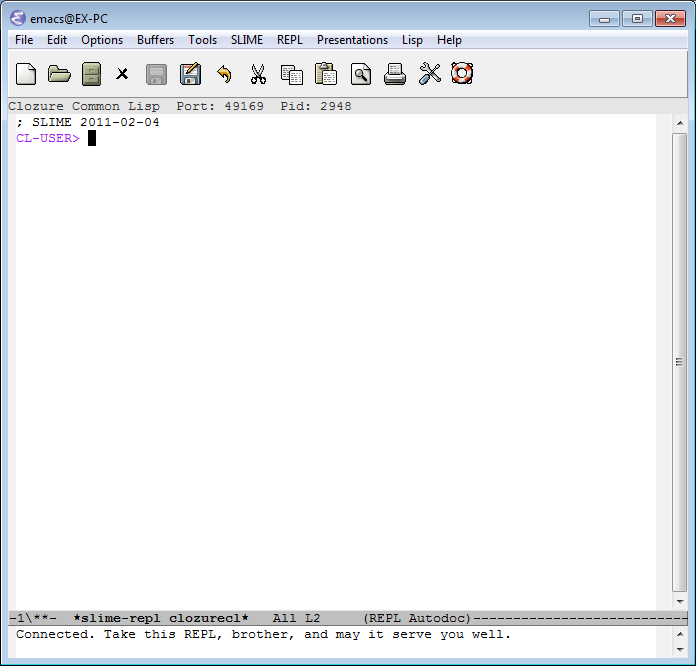
\includegraphics[scale=.6]{lispbox_started}\\
  \small{\textit{Запущенный lispbox}}
\end{center}
\subsection{Работа в lispbox}
Lispbox, как и любая приличная IDE для Лиспа, обладает тремя облегчающими жизнь опциями:
\begin{itemize}
\item ведет подсчет открывающих и закрывающих скобок --- при постановке закрывающей скобки подсвечивается соответсвтующая открывающая
\item автоматически выравнивает исходный код (по нажатию клавиши Tab) как в режиме интерпретатора, так и в режиме редактирования исходного кода
\item подсвечивает исходный код
\end{itemize}
Помимо перечисленного выше, у lispbox есть еще множество особенностей, со многими из которых мы познакомимся позднее.

Emacs --- основа выбранной нами IDE --- крайне гибкий и мощный инструмент, однако, довольно требовательный к пользователю. Безграничный потенциал Emacs и его отличия от традиционных текстовых редакторов породили множество легенд о сложности в освоении и использовании. Но это совсем не так. Совершим небольшой экскурс по основным понятиям и командам Emacs.
\subsubsection{Буфер}
\textit{Буфером} называется во-первых любой открытый файл, а во-вторых вообще любое пространство, в которое вводится или выводится информация. Название буфера пишется внизу слева. Все буферы перечислены в верхнем меню Buffer. Как видно, после старта lispbox по умолчанию открыты буферы под названиями \verb|*scratch*|, \verb|*Messages*|, \verb|*slime-events*|, \verb|*slime-repl clozurecl*| и \verb|*inferior-lisp*|. Первые два являются стандартными буферами Emacs, следующие два --- служебные буферы Slime, и наконец последний --- интерпретатор, открытый сейчас перед нами. Обратите внимание на название буфера, написанное слева внизу.
\begin{center}
  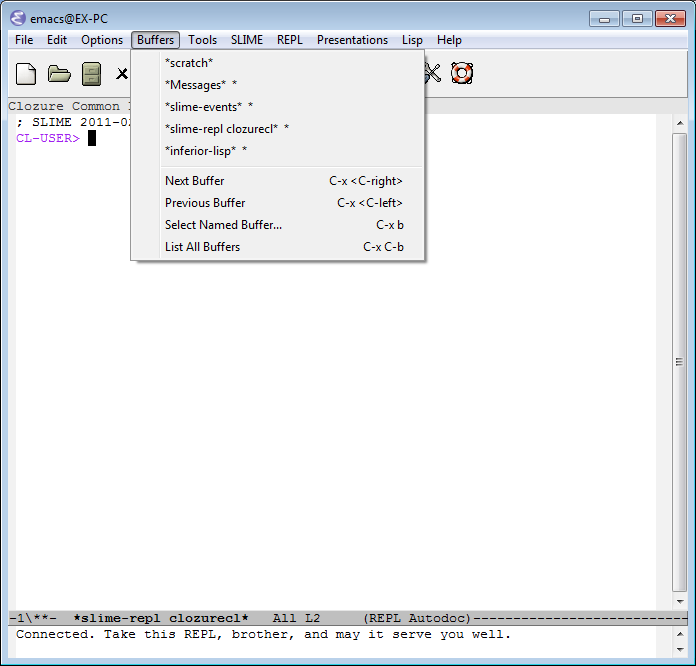
\includegraphics[scale=.6]{lispbox_buffers}\\
  \small{\textit{Буферы по умолчанию}}
\end{center}
\subsubsection{Горячие клавиши}
На рисунке выше внизу выпадающего меню рядом с командами находятся сочетания клавиш, также иногда называемые аккрдами, назначенные на эти команды.
Такие сочетания используются в Emacs повсеместно, и после некоторого привыкания очень сильно облегчают работу. Однако, конвенция, принятая в Emacs, довольно сильно отличается от всех остальны программ, и требует пояснения.

Рассмотрим, к примеру, команду \texttt{Previous buffer}. Как видно из скиншота выше, этой команде назначено сочетание \verb|C-x <C-left>|. Буквой С в Emacs обозначается нажатие на клавишу Control. Запись \texttt{C-x} обозначает всего-навсего сочетание Control-x. Последовательность \verb|C-x <C-left>| же означает, что сначала нужно набрать Control-x, а потом Control-<стрелка влево>. Сделать это можно и не отпуская клавишу Control, то есть зажать Control, потом нажать и отпустить x, а потом нажать стрелку влево.
Если префикс \verb|С-| не указан, значит нажатие на Control не нужно. То есть \verb|С-х b| означает нажатие Control-x, за которым следует нажатие на b уже при отпущенной клавише Control. Также существуют сочетания с клавишей Alt, которые записываются как \verb|M-| (от названия клавиши Meta, отсутствующей на современных клавиатурах).
Основные команды работы с буферами, многие из которых также доступны через меню ``File'' и ``Buffers'', перечислены ниже:
\begin{itemize}
\item \verb|C-x C-f| открывает файл с с введенным именем. Если файл есть, открывает для редактирования, если нет --- создает новый
\item \verb|C-x b| <имя буфера> переключается на буфер с введенным именем. Если такого буфера нет, то он будет создан 
\item \verb|C-x C-b| создает новое \textit{окно}, в которое выводит список существующих буферов
\item \verb|C-x <C-left>| и \verb|C-x <C-right>| переключает окно на предыдущий/следующий буфер. Тот же самый эффект имеет щелчок ЛКМ/ПКМ по имени буфера
\item \verb|C-x k| закрывает буфер, в котором находится курсор. Если буфер остался один, закрыть его нельзя. Если вы попытаетесь закрыть буфер, открытый на файле, и имеющий несохраненные данные, Emacs попросит подтверждения выполнения
\item \verb|C-x C-s| сохраняет содержимое буфера в текстовый файл
\end{itemize}
\subsubsection{Окна}
Emacs использует термин ``окно'' в несколько отличном от привычного смысле. Окно в том же смысле, в котором его используем мы, то есть в смысле отдельного окна опрерационной системы, в Emacs называется \textit{фреймом}. Окном же называется область, в которой отображается ровно один буфер. Новые окна можно получить, деля существующие по горизонтали или по вертикали. Две команды для работы с окнами можно найти в меню ``File''. Некоторые команды для работы с окнами:
\begin{itemize}
\item \verb|C-x 2| делит окно по горизонтали
\item \verb|C-x 3| делит окно по вертикали
\item \verb|C-x 0| закрывает окно, в котором находится курсор, сливая его с ближайшим соседним окном. Как и в случае с буфером, закрыть последнее открытое окно нельзя. Обратите внимание, что буфер, отображавшийся в окне, никуда не пропадает, и вернуться к нему можно при помощи команды C-x b
\item \verb|C-x 1| разворачивает выбранное окно на весь фрейм. Также это можно трактовать как закрытие всех окон, кроме выбранного
\item \verb|C-x o| переносит курсор в следующее окно. Также окна можно выбирать при помощи мыши
\end{itemize}
\subsubsection{Работа с текстом}
\begin{itemize}
\item \verb|<C-space>| начинает выделение текста, аналогично обычному выделению мышью
\item \verb|C-w| вырезает выделенный текст (на самом деле, команда работает несколько сложнее, но чаще всего используется именно для вырежания выделенного текста)
\item \verb|M-w| копирует выделенный текст
\item \verb|C-y| вставляет текст из буфера обмена. Если после нажатия \verb|C-y| нажать \verb|M-y|, вставится предпоследний скопированный (или вырезанный) текст. Это удобно, например, для того, чтобы поменять местами два слова
\item \verb|C-/| отменяет последнее действие
\item \verb|C-p| и \verb|C-n| переход на предыдущую/следующую строку (стрелки вверх и вниз)
\item \verb|C-f| и \verb|C-b| переход на символ вперед/назад (стрелки вправо и влево)
\item \verb|C-a| и \verb|C-e| переход в начало/конец строки (клавиши Home и End)
\item \verb|M-f| и \verb|M-b| переход на слово вперед/назад
\item \verb|M-| вырезает слово после курсора (до пробела или спецсимвола)
\item \verb|<M-backspace>| вырезает слово перед курсором (до пробела или спецсимвола)
\end{itemize}
\subsection{Интерпретатор}
Итак, среда запущена и готова к работе. Вы видите перед собой приглашение, гласящее \verb|Cl-USER>|. Такой режим работы Лиспа называется REPL --- Read-Eval-Print Loop, также известный как интерактивный режим или \textit{toplevel}. Суть его заключается в том, что пользователь напрямую общается с лисп-системой, производя вычисления и получая ответы в реальном времени. Этот режим, впервые появившийся в Лиспе, отличает его от статических, компилируемых языков типа Фортрана, С или Java, и присутствует практически во всех динамических языках, например Ruby, Python и Perl. Несмотря на то, что этот режим присущ интерпретируемым языкам, почти все современные реализации Common Lisp являются компилируемыми, и Clozure CL в этом плане не исключение.

Числа и строки являются самыми простыми выражениями, доступными программисту, и вычисляются сами в себя. Поприветствуйте lispbox, введя в строке приглашения что-нибудь вроде \verb|"Привет, Лисп!"|, и нажав Enter. Строка, введенная вами, выведется на экран, а после неё снова появится строка приглашения. То же самое произойдет, если вводить числа, простые и десятичные дроби, а также некоторые другие выражения:
\begin{center}
  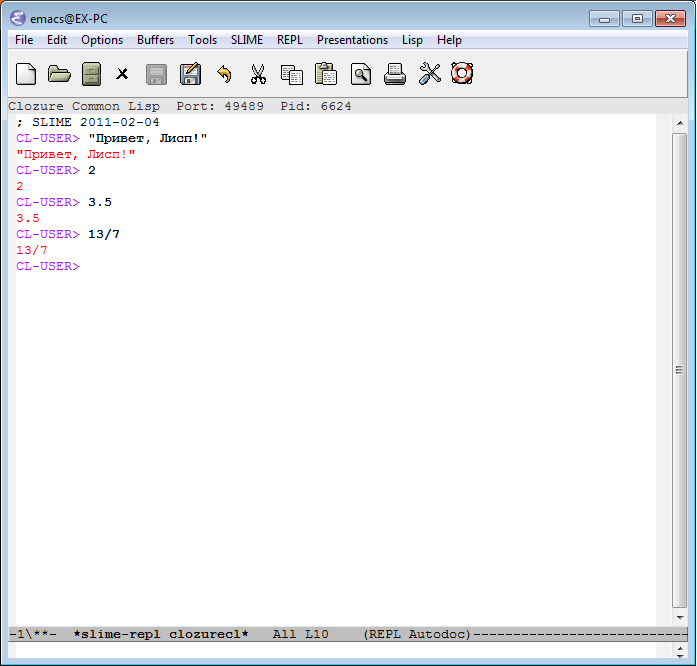
\includegraphics[scale=.7]{lispbox_toplevel}\\
  \small{\textit{Простейшие выражения}}
\end{center}
Теперь рассмотрим более сложные примеры команд. Например, если мы хотим сложить два числа 1 и 2, следует ввести \verb|(+ 1 2)|. Как несложно заметить, такая запись несколько отличается от принятой и в математике, и в других языках программирования. Это непривычно, однако более универсально: для записи сложения трех чисел обычная запись требует использования уже двух знаков ``+'', в то время как в префиксной нотации, принятой в Лиспе, сложение трех чисел будет выглядеть так: \verb|(+ 1 2 3)|. Таким образом, операция сложения может принимать произвольное количество агрументов, а может и не принимать ни одного арумента вообще. Умножение работает точно таким же образом. Вычитание и деление отличаются тем, что должны принимать хотя бы один агрумент --- соответственно, уменьшаемое и делимое.

Выражения могут быть вложенными: \verb|(+ (* 2 3 4) (/ 10 3))|. Так как количество агрументов может быть произвольным, скобки служат для обозначения границ выражений. Выражения Лиспа также называются \textit{формами}. В дальнейшем будем считать эти термины синонимами. % А на самом деле они синонимичны?
Большие формы с глубокой вложенностью удобно записывать, разбивая на несколько строк, каждую из которых можно выровнять нажатием на клавишу Tab.
\begin{center}
  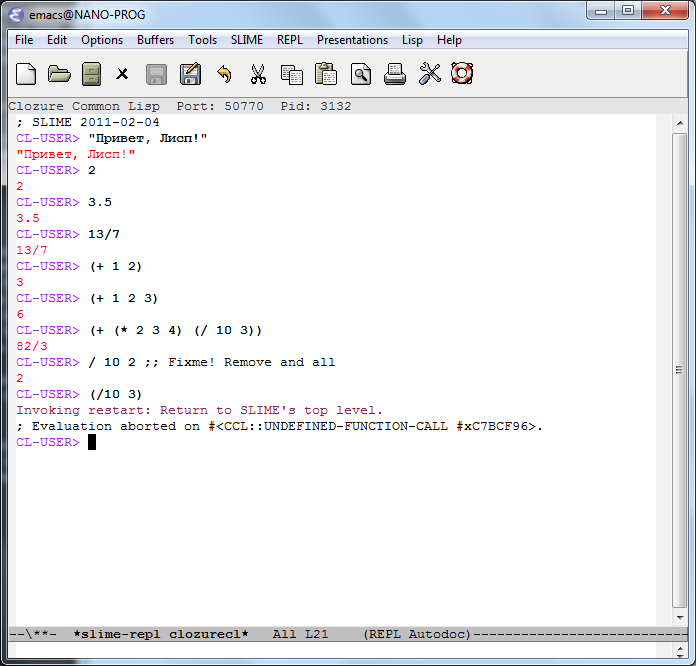
\includegraphics[scale=.7]{lispbox_more_complex}\\ %Тут обязательно надо что-то со вложенностью и примером выравнивания форм
  \small{\textit{Более сложные формы}}
\end{center}
\subsubsection{Ошибки}
Если вы допустите какую-либо ошибку, lispbox остановит выполнение вычисления и сообщит вам о найденном несоотвествии. Помимо вывода информации о том, что за ошибка произошла, и чему в этот момент были равны значения переменных, lispbox поинтересуется, что делать дальше. В подавляющем большинстве вариантов нас будет интересовать вариант \verb|[*ABORT]|, возвращающий нас к строке приглашения. Он будет перечислен в списке вариантов под определённым номером, но удобнее воспользоваться горячей клавишей \verb|q|, нажатие на которую вернёт нас из списка возможных рестартов в интерпретатор.
\begin{center}
  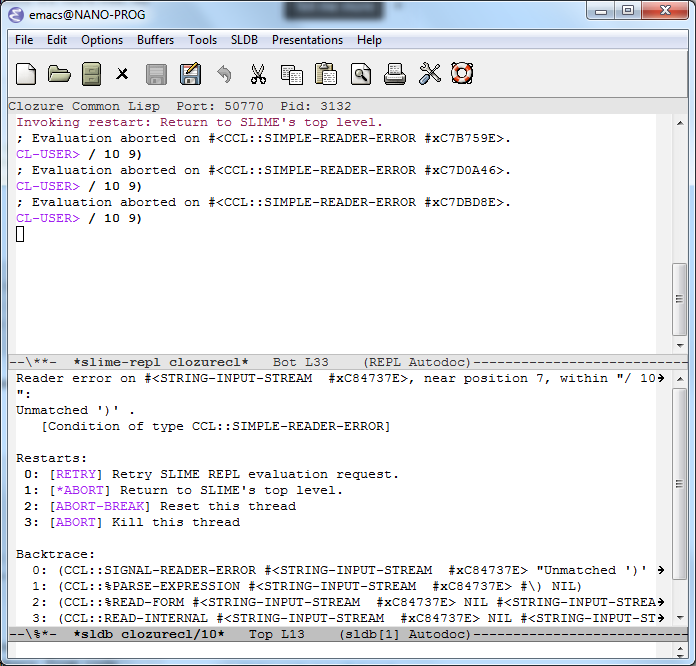
\includegraphics[scale=.7]{lispbox_error_conditions}\\
  \small{\textit{Сообщение об ошибке и список\\возможных вариантов развития событий}}
\end{center}
\subsubsection{Задание 1}
Запишите на Лиспе следующее арифметическое выражение:\\
\[
\cfrac{((24 - 12) + (6 - 3))\cdot\cfrac{6.9 - 3.2}{((4 - 1)\cdot(4 + 1)\cdot(4 - 5))}}{13 - 5}
\]
\newpage
\section{Основы Лиспа}
В этом разделе будут подробно рассмотрены общие для всех диалектов выразительные средства, неизменные с 1956-го года и присутствующие в любом диалекте Лиспа, существующем в наши дни. Также некоторое внимание будет уделено обзору расширений этой базовой модели, присутствующих в стандарте Common Lisp.
\subsection{Типы данных}
Все типы данных, с которыми может работать Лисп, можно разделить на две глобальные группы --- простые и составные. 
\subsubsection{Простые типы}
Простые типы данных, также называемые атомарными, с свою очередь делятся на числовые и символьные. Значение считается числовым, если начинается с цифры, знаков \verb|+|  или \verb|-|, и записано в обычной для чисел форме. Все остальные значения являются символьными. В записи символа можно использовать буквы, цифры, и спецсимволы, но есть несколько ограничений: символы не могут начинаться со знака \verb|#|. С этого знака начинаются \textit{макросы чтения}, используемые для записи значений большинства составных и некоторых атомарных типов данных. Макросы чтения будут рассмотрены позднее. % Или не будут
Также в названиях символов нельзя использовать знаки \verb|( ) " ' ` , : ;|. Регистр букв в записи не имеет значения: \verb|eyem-the-strongest| и \verb|eyem-the-STRONGEST| --- две разные записи одного и того же символа. Если мы хотим включить в название символа специальные символы или пробелы, то его надо заключить в вертикальные черты: \verb#|служебные знаки:( , ; :)|#. Это также сделает символ чувствительным к регистру.

Символы используются для записи имен переменных и функций.
\begin{itemize}
  \renewcommand{\labelitemii}{$\bullet$}
\item[] Примеры числовых значений:
  \begin{itemize}
  \item \verb|10|
  \item \verb|-23.5|
  \item \verb|+44/13|
  \end{itemize}
\item[] Примеры символьных значений:
  \begin{itemize}
  \item \verb|x|
  \item \verb|кошачья-мята|
  \item \verb|*|
  \item \verb|+-10|
  \item \verb|+43/-32|
  \item \texttt{20.05.15}
  \item \verb|cack315#1ie|
  \item \verb|@#$%!|
  \item \begin{CJK}{UTF8}{min}\verb|窓月|\end{CJK} % не компилируется в виндоузе!
  \item \verb#|электрификация южных губерний|#
  \end{itemize}
\end{itemize}
Среди всех символов, возможных в Лиспе, два являются особыми --- это специальные константы \verb|T| и \verb|NIL|, обозначающие логические значения \textit{true} и \textit{false}. \verb|NIL| также обозначает пустой список. 

Стоит отметить, что чаще всего символы используются для обозначения переменных и функций, и имеют имена вроде \texttt{x}, \texttt{y}, \texttt{search-rb-tree} или \texttt{*global-state-pool*}. Примеры, приведенные выше, хотя и являются примерами валидных символов, в реальном мире встречаются очень редко и в исключительных случаях.

Кроме целых чисел, дробей, и числе с плавающей точкой в Common Lisp существуют также комплексные числа. Записываются они следующим образом: \texttt{\#C(2.7 3/5)}, что соответствует комплексному числу \(2.7+\cfrac{3}{5}\cdot{}i\).

К атомарным типам относится также \textit{символьный тип} (character), который не следует путать с символом (symbol). Значения символьного типа --- глифы различных алфавитов, иероглифы и прочие символы, поддерживаемые Юникодом, например: \texttt{\#\textbackslash{}Q} --- большая английская буква q.
\subsubsection{Составные типы}
Простейшим из всех составных типов является \textit{список}. Он же является одним из ключевых понятий Лиспа. Собственно, название LISP появилось как акроним от выражения \textbf{lis}t \textbf{p}rocessor --- обработчик списков.

Самый простой возможный список --- пустой. Он записывается как \verb|nil| или \verb|'()|. Списки могут содержать как атомы, так и другие списки и иные составные типы данных. Некоторые примеры списков:
\begin{itemize}
  \item \begin{alltt}(a \(\lambda\) 4.5 33/7)\end{alltt}
  \item \verb|((9 3.7) () (a b) nil)|
  \item \verb|()|
\end{itemize}
Сам код программы тоже записывается в виде списка. Это одно из важнейших свойств Лиспа, из которого вытекает множество интересных последствий, и благодаря которому Лисп заслужил звание программируемого языка программирования.

Другие составные типы данных, доступные в языке Common Lisp (некоторые из них будут рассмотрены позднее):
\begin{itemize}
\item Векторы (включая строки и битовые векторы)
\item Многомерные массивы
\item Структуры
\item Классы
\end{itemize}
\subsection{Вычисление}
Как говорилось ранее, программа, записанная на Лиспе, представляет собой список. Любая более-менее сложная программа (содержащая больше одной формы), является набором вложенных форм. Напомним, форма --- это выражение, а в Лиспе каждое выражение можно вычислить. Всего в Лиспе есть три типа вычислимых выражений.
\begin{enumerate}
\item Числа, и константные символы вычисляются сами в себя. Common Lisp добавляет к ним также значения символьного типа и строки:
  \begin{itemize}
  \item[] \begin{alltt}42 \(\longrightarrow\) 42\end{alltt}
  \item[] \begin{alltt}88/14 \(\longrightarrow\) 44/7\end{alltt}
  \item[] \begin{alltt}"Hello, Lisp" \(\longrightarrow\) "Hello, Lisp"\end{alltt}
  \item[] \texttt{\#\textbackslash{}ц $\longrightarrow$ \#\textbackslash{}ц}
  \item[] \begin{alltt}nil \(\longrightarrow\) NIL\end{alltt}
  \item[] \begin{alltt}() \(\longrightarrow\) NIL\end{alltt}
  \item[] \begin{alltt}T \(\longrightarrow\) T\end{alltt}
  \end{itemize}
\item Обычные символы можно вычислить только тогда, когда он является именем какой-то переменной. Механизмы связывания имени переменной с её значением рассмотрим чуть позднее. Если с символом связано некоторое значение, то он вычисляется следующим образом:
  \begin{itemize}
  \item[] \begin{alltt} x \(\longrightarrow\) (A 3 (4 BETA))\end{alltt}
  \item[] \begin{alltt} некий-символ \(\longrightarrow\) 42\end{alltt}
  \end{itemize}
\item Список можно вычислить, если он представляет собой \textit{функциональный вызов} --- то есть его первым элементом является символ, с которым связана определенная функция. Про то, как назначить символу функцию, то есть \textit{определить функцию}, будет рассказано в следующей главе. Пример функционального вызова:
  \begin{itemize}
  \item[] \texttt{(f e\textsubscript{1} e\textsubscript{2} $\ldots$ e\textsubscript{n})}, где
    \begin{itemize}
    \item[] \verb|f| --- символ, с которым связана функция
    \item[] \verb|n| $\ge$ 0 --- количество агрументов функции
    \item[] \texttt{e\textsubscript{1} e\textsubscript{2} $\ldots$ e\textsubscript{n}} --- аргументы функции
    \end{itemize}
  \end{itemize}
  Если с \texttt{f} не связана никакая функция, Лисп выдаст сообщение об ошибке.
\end{enumerate}
Так как аргументы тоже являются формами, им может потребоваться вычисление. Поэтому перед тем, как вызвать функцию, вычисляются значения всех её аргументов. Однако есть некоторые функции, нарушающие это правило. Такие функции называются \textit{специальными}. Их в языке меньшинство, и при дальнейшем рассмотрении, если функция является специальной, это будет указаываться явно. У пользователя есть возможность создавать как обычные так и специальные функции.
\subsection{Базовые функции Лиспа}
Основу любого диалекта Лиспа составляют 8 функций:
\begin{itemize}
\item[] Три для работы со списками: \texttt{car}, \texttt{cdr} и \texttt{cons}
\item[] Два предиката: \texttt{atom}, \texttt{eq}
\item[] Две функции для контроля процесса вычисления: \texttt{quote} и \texttt{eval}
\item[] Функция для контроля потока выполнения: \texttt{cond}
\end{itemize}
\subsubsection{\lisp{cons}}
Обыкновенная функция. Она принимает два аргумента и конструирует из них \textit{cons-ячейку}. Если вторым аргументом \lisp{cons} является список, то в результате получится тоже список:
\begin{examples}
  \item \lisp{(cons 'a 'b)} $\longrightarrow$ \lisp{'(a . b)}
  \item \lisp{(cons 'a '(c d e))} $\longrightarrow$ \lisp{'(a c d e)}
\end{examples}
\subsubsection{\lisp{car}}
Обыкновенная функция. Принимает в качестве аргумента cons-ячейку и возвращает её левую часть. Если cons-ячейка является списком, возвращает первый элемент списка. Полное название функции --- contents of address register.
\begin{examples}
\item \lisp{(car '(1 . 2))} $\longrightarrow$ \lisp{1}
\item \lisp{(car '(foo bar qux)} $\longrightarrow$ \lisp{foo}
\end{examples}
\subsubsection{\lisp{cdr}}
Обыкновенная функция. Принимает cons-ячейку и возвращает правую её часть. Если аргумент --- список, то функция возвращает все его элементы, кроме первого. Название происходит от ``contents of decrement register''.
\begin{examples}
\item \lisp{(cdr '(3 . 42)} $\longrightarrow$ \lisp{42}
\item \lisp{(cdr '(альфа бета гамма)} $\longrightarrow$ \lisp{(БЕТА ГАММА)}
\end{examples}
\subsubsection{\lisp{atom}}
Обыкновенная функция. Принимает любой аргумент, возвращает \lisp{T}, если аргумент является атомом, и \lisp{NIL} в противном случае.
\begin{examples}
\item \lisp{(atom '(1 2 3))} $\longrightarrow$ \lisp{NIL}
\item \lisp{(atom '(a . b)} $\longrightarrow$ \lisp{NIL}
\item \lisp{(atom t)} $\longrightarrow$ \lisp{T}
\item \lisp{(atom nil)} $\longrightarrow$ \lisp{T}
\item \lisp{(atom 'a)} $\longrightarrow$ \lisp{T}
\end{examples}
\subsubsection{\lisp{eq}}
Обыкновенная функция. Принмает два аргумента и возвращает \lisp{T}, если это они указывают на один и тот же объект (в терминах машинных команд). Стоит сказать, что два символа считаются одинаковыми, если у них одинкавые имена. Разные списки же, как и другие составные объекты, даже если и содержат одни и те же элементы, занимают разное место в оперативной памяти и поэтому считаются разными.
\begin{examples}
\item \lisp{(eq 1 2)} $\longrightarrow$ \lisp{NIL}
\item \lisp{(eq 4 4)} $\longrightarrow$ \lisp{T}
\item \lisp{(eq () nil)} $\longrightarrow$ \lisp{T}
\item \lisp{(eq '(1 2) '(1 2))} $\longrightarrow$ \lisp{NIL}
\item \lisp{(eq 'b 'b)} $\longrightarrow$ \lisp{T}
\end{examples}
\subsubsection{\lisp{quote}}
Специальная функция. Принимает свой аргумент и возвращает его, не вычисляя. Настолько активно применяется в Лиспе, что для неё существует специальное сокращение --- \lisp{'}, при таком использовании скобки вокруг аргумента опускаются: запись \lisp{(quote (a 1 2))} эквивалентна записи \lisp{'(a 1 2)}. Запись полного имени функции пратически не используется. Также называется функцией блокировки вычислений.
\begin{examples}
\item \lisp{(quote b)} $\longrightarrow$ \lisp{b}
\item \lisp{(quote (+ 1 2 3))} $\longrightarrow$ \lisp{(+ 1 2 3)}
\item \lisp{(quote (car '(a b c)))} $\longrightarrow$ \lisp{(CAR '(A B C))}
\item \lisp{'(a b c)} $\longrightarrow$ \lisp{(a b c)}
\item \lisp{'foobar} $\longrightarrow$ \lisp{foobar}
\end{examples}
\subsubsection{\lisp{eval}}
Обыкновенная функция. Принимает свой аргумент и вычисляет его два раза. Может использоваться для снятия блокировки вычислений, установленной функцией \lisp{quote}, а также для вычисления результата вычисления своего аргумента, если он является функциональным вызовом. В практике Common Lisp не используется практически никогда.
\begin{examples}
\item \lispex{(eval (quote (atom q)))}{T}
\item \lispex{(eval '(car '(a b c)))}{A}
\item \lispex{(eval ''c)}{C}
\item \lispex{(eval (cons 'car '('(a b c))))}{A}
\end{examples}
\subsubsection{\lisp{cond}}
Специальная функция. Служит для разветвления вычислений. Принимает ноль и более агрументов вида \lisp{(b f\textsubscript{1} f\textsubscript{2} \ldots f\textsubscript{n})}, где \lisp{b} --- форма, значением которой является 
\end{document}
